\documentclass{beamer}
  \usepackage[czech]{babel}
  \usepackage[utf8]{inputenc}
  \usepackage[IL2]{fontenc}
  \usepackage{textcomp}
  \usepackage{color}
  \usepackage{algorithm,algorithmic}
  \usepackage{epstopdf}

  \usetheme{Boadilla}
  \usecolortheme{beaver}

  \graphicspath{ {./fig/} }

  \title[Porovnání]{Porovnání\ --\ vyhledání silně souvislých komponent}
  \subtitle{Gabowův algoritmus a Tarjanův algoritmus}
  \author[Wrona, Varga]{Jan~Wrona \and Tomáš~Varga}
  \institute[FIT VUT]
  {
    Fakulta informačních technologií\\
    Vysoké učení technické v Brně
  }
  \date[GAL 2014]{Grafové algoritmy, 2014}

  \beamertemplatenavigationsymbolsempty

  \AtBeginSection[]
  {
    \begin{frame}
    \frametitle{Obsah}
    \tableofcontents[currentsection]
    \end{frame}
  }
  \AtBeginSubsection[]
  {
    \begin{frame}
    \frametitle{Table of Contents}
    \tableofcontents[currentsection,currentsubsection]
    \end{frame}
  }

\begin{document}

\frame{\titlepage}

\section{Algoritmy}
\begin{frame}{Gabowův algoritmus}
\begin{algorithm}[H]
\algsetup{linenosize=\tiny}
\scriptsize
\begin{algorithmic}
  \STATE $preorder[v] \leftarrow c;\ c \leftarrow c + 1;\ push(S, v);\ push(P, v)$
  \FOR{$w$ in $Adj[v]$}
    \IF{$preorder[w]=\infty$}
      \STATE{GABOW-VISIT($w$)}
    \ELSIF{$w$ is in $S$}
      \REPEAT
        \STATE{$pop(P)$}
      \UNTIL{$preorder[peak(P)] \leq preorder[w]$}
    \ENDIF
  \ENDFOR

  \bigskip

  \IF{$v=peak(P)$}
    \STATE{vytvoř novou silně souvislou komponentu $c$}
    \REPEAT
      \STATE{$w \leftarrow pop(S)$}
      \STATE{přidej $w$ do komponeny $c$}
    \UNTIL{$v=w$}
    \STATE{$pop(P)$}
    \STATE{$return\ c$}
  \ENDIF
\end{algorithmic}
\caption{Funkce GABOW-VISIT(v).}
\label{alg:gabow}
\end{algorithm}
\end{frame}

\begin{frame}{Tarjanův algoritmus}
\begin{algorithm}[H]
\algsetup{linenosize=\tiny}
\scriptsize
\begin{algorithmic}
  \STATE $index[v] \leftarrow index;\ lowlink[v] \leftarrow index;\ index \leftarrow index + 1;\ push(S, v)$
  \FOR{$w$ in $Adj[v]$}
    \IF{$index[w]=\infty$}
      \STATE{TARJAN-VISIT($w$)}
    \ELSIF{$w$ is in $S$}
      \STATE{$lowlink[v] \leftarrow min(lowlink[v], index[w])$}
    \ENDIF
  \ENDFOR

  \bigskip

  \IF{$lowlink[v]=index[v]$}
    \STATE{vytvoř novou silně souvislou komponentu $c$}
    \REPEAT
      \STATE{$w \leftarrow pop(S)$}
      \STATE{přidej $w$ do komponeny $c$}
    \UNTIL{$v=w$}
    \STATE{$return\ c$}
  \ENDIF
\end{algorithmic}
\caption{Funkce TARJAN-VISIT(v).}
\label{alg:tarjan}
\end{algorithm}
\end{frame}

\begin{frame}{Asymptotická časová složitost}
\begin{itemize}
\item Reprezentace seznamem sousedů.
\bigskip
\item \textbf{Gabowův} a \textbf{Tarjanův}: upravené DFS. První průchod $O(m+n)$, druhý průchod $O(n)$.
\item \textbf{Tarjanův} s \textbf{Nuutilovou} modifikací: upravený pouze druhý průchod, zlepšení složitosti pro řídké grafy.
\item \textbf{Kosarajův}: dva kompletní průchody grafem, transpozice, složitost $\Theta(m+n)$.
\end{itemize}
\end{frame}

\section{Implementace a testování}
\begin{frame}{Implementace}
\begin{itemize}
\item Python2.
\item Knihovny \emph{NetworkX}, \emph{psutil}.
\item \emph{NetworkX} nepřipouští smyčky v orientovaném grafu.
\bigskip
\item \textbf{Gabowův} a \textbf{Tarjanův}: vlastní implementace i reprezentace grafu.
\item \textbf{Tarjanův} s \textbf{Nuutilovou} modifikací a \textbf{Kosarajův}: součást knihovny NetworkX.
\end{itemize}
\end{frame}

\begin{frame}{Návrh testů}
\begin{algorithm}[H]
\algsetup{linenosize=\tiny}
\scriptsize
\begin{algorithmic}
  \FOR{$i \leftarrow 1 $ to $repetitions$}
    \STATE{$startTime \leftarrow cpuTime$}
    \STATE{$startMemory \leftarrow memory$}
    \FOR{$j \leftarrow 1 $ to $multiplication$}
      \STATE{SCC-ALGORITHM(G)}
    \ENDFOR
    \STATE{$totalTime \leftarrow cpuTime - startTime$}
    \STATE{$totalMemory \leftarrow memory - startMemory$}
  \ENDFOR
\end{algorithmic}
\caption{Metoda měření.}
\label{alg:measurement}
\end{algorithm}

\begin{itemize}
\item Vnější cyklus zmenšuje chybu měření\ --\ výběr minima z naměřených časů.
\item Vnitřní cyklus eliminuje nízké rozlišení měřeného procesorového času.
\end{itemize}
\end{frame}

\begin{frame}{Způsob měření času a paměti}
\begin{itemize}
\item Čas měřen pomocí \texttt{time.clock()}. Jedná se o procesorový čas v sekundách.
\bigskip
\item Paměť měřena pomocí metody \texttt{memory\_info()} třídy \texttt{Process} knihovny \emph{psutil}.
\item \texttt{memory\_info()} zjistí velikost fyzické paměti využité procesem\ --\ resident set size.
\end{itemize}
\end{frame}

\section{Výsledky experimentů}
\subsection{Jednotlivé algoritmy\ --\ časová složitost}
\begin{frame}{Gabowův algoritmus}
  \includegraphics[width=\textwidth,height=\textheight,keepaspectratio]{gabow}
\end{frame}
\begin{frame}{Tarjanův algoritmus}
  \includegraphics[width=\textwidth,height=\textheight,keepaspectratio]{tarjan}
\end{frame}
\begin{frame}{Tarjanův algoritmus s Nuutilovou modifikací}
  \includegraphics[width=\textwidth,height=\textheight,keepaspectratio]{tarjan_nx}
\end{frame}
\begin{frame}{Kosarajův algoritmus}
  \includegraphics[width=\textwidth,height=\textheight,keepaspectratio]{kosaraju_nx}
\end{frame}

\subsection{Srovnání algoritmů\ --\ časová složitost}
\begin{frame}{Srovnání\ --\ řídký graf}
  \includegraphics<1>[width=\textwidth,height=\textheight,keepaspectratio]{0_2}
  \includegraphics<2>[width=\textwidth,height=\textheight,keepaspectratio]{0_2_no_kosa}
\end{frame}
\begin{frame}{Srovnání\ --\ vyvážený graf}
  \includegraphics<1>[width=\textwidth,height=\textheight,keepaspectratio]{0_5}
  \includegraphics<2>[width=\textwidth,height=\textheight,keepaspectratio]{0_5_no_kosa}
\end{frame}
\begin{frame}{Srovnání\ --\ hustý graf}
  \includegraphics<1>[width=\textwidth,height=\textheight,keepaspectratio]{0_8}
  \includegraphics<2>[width=\textwidth,height=\textheight,keepaspectratio]{0_8_no_kosa}
\end{frame}
\begin{frame}{Srovnání\ --\ úplný graf}
  \includegraphics<1>[width=\textwidth,height=\textheight,keepaspectratio]{1_0}
  %\includegraphics<2>[width=\textwidth,height=\textheight,keepaspectratio]{1_0_no_kosa}
\end{frame}

\subsection{Jednotlivé algoritmy\ --\ prostorová složitost}
\begin{frame}{Gabowův algoritmus}
  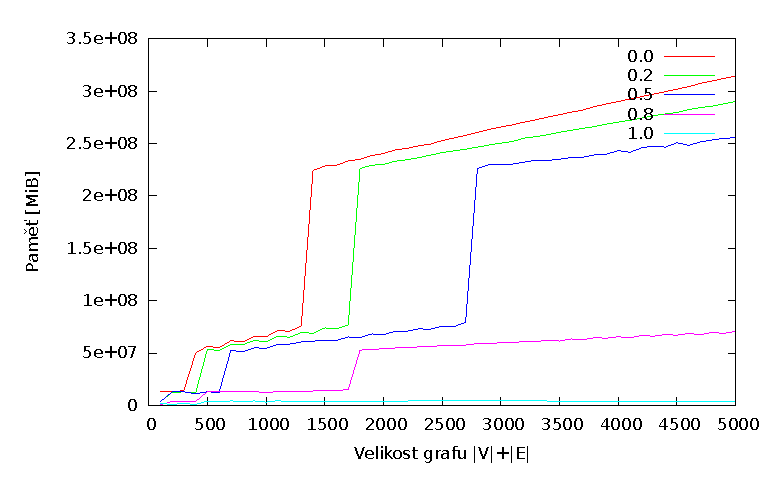
\includegraphics[width=\textwidth,height=\textheight,keepaspectratio]{gabow_memory}
\end{frame}
\begin{frame}{Tarjanův algoritmus}
  \includegraphics[width=\textwidth,height=\textheight,keepaspectratio]{tarjan_memory}
\end{frame}

\subsection{Srovnání algoritmů\ --\ prostorová složitost}
\begin{frame}{Srovnání\ --\ řídký graf}
  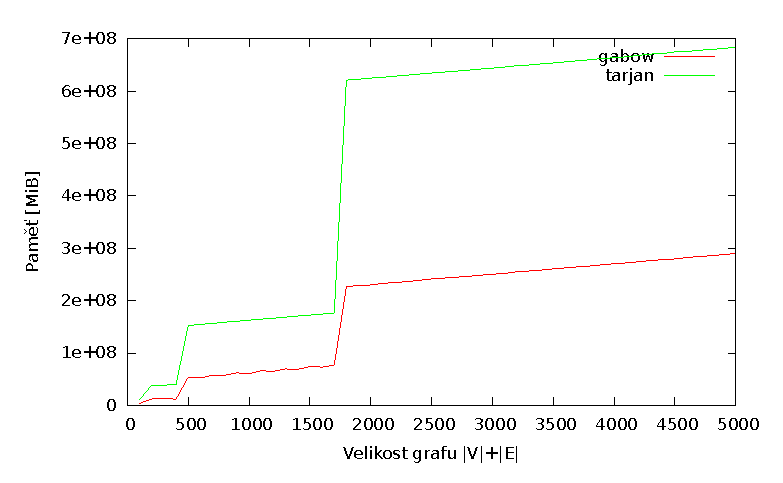
\includegraphics[width=\textwidth,height=\textheight,keepaspectratio]{0_2_memory}
\end{frame}
\begin{frame}{Srovnání\ --\ hustý graf}
  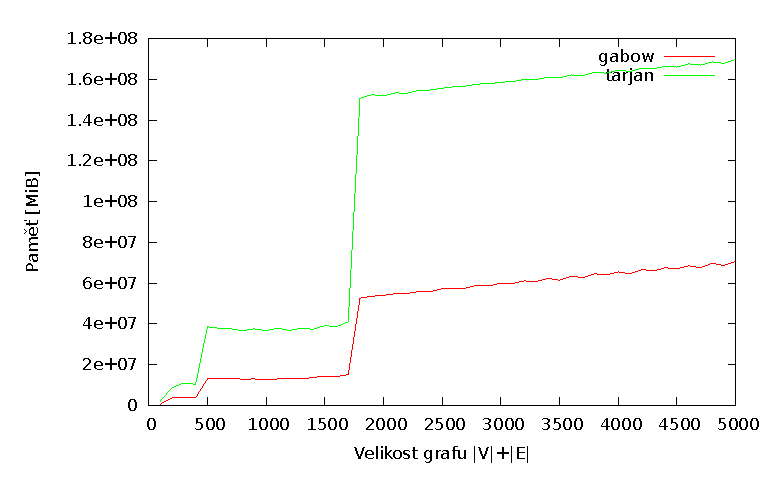
\includegraphics[width=\textwidth,height=\textheight,keepaspectratio]{0_8_memory}
\end{frame}

\end{document}
